% Main file for Overleaf: Assignment06_Report.tex
% V02. Compile with pdfLaTeX or Tectonic; generated evidence tables are reproducible.
% Keep figures/ beside this source. Optional cover logo: bia.png.
\documentclass[12pt,a4paper]{article}
\usepackage{iftex}
\ifPDFTeX
\usepackage[utf8]{inputenc}
\usepackage[T5]{fontenc}
\usepackage{lmodern}
\else
\usepackage{fontspec}
\setmainfont{LiberationSerif}[Path=fonts/,Extension=.ttf,UprightFont=*-Regular,BoldFont=*-Bold,ItalicFont=*-Italic,BoldItalicFont=*-BoldItalic]
\fi
\usepackage[english]{babel}
\usepackage{geometry}
\geometry{top=2cm,bottom=2cm,left=2.2cm,right=2.2cm}
\usepackage{graphicx,float,longtable,array,booktabs,enumitem,xcolor,hyperref,setspace,parskip}
\usepackage{amsmath,tabularx,listings,caption,placeins,microtype}

\hypersetup{colorlinks=true,linkcolor=black,urlcolor=blue,pdftitle={Assignment 06 -- Multimodal Search System for E-Commerce},pdfauthor={Đào Văn Khang}}
\setlength{\parindent}{0pt}
\setlength{\parskip}{0.35em}
\setstretch{1.5}
\renewcommand{\arraystretch}{1.25}
\setlength{\emergencystretch}{3em}
\newcolumntype{L}{>{\raggedright\arraybackslash}X}
\newcommand{\code}[1]{\texttt{#1}}
\captionsetup{font=small,labelfont=bf}
\setlist{itemsep=2pt,topsep=5pt}
\lstset{basicstyle=\ttfamily\footnotesize,breaklines=true,columns=fullflexible,keepspaces=true,frame=single,backgroundcolor=\color{black!3},showstringspaces=false,tabsize=4,captionpos=b}
\pagestyle{plain}

\newcommand{\StudentName}{ĐÀO VĂN KHANG}
\newcommand{\StudentID}{B23DCVT218}
\newcommand{\StudentClass}{E23TTNT01}
\newcommand{\StudentGroup}{04}
\newcommand{\LecturerName}{Assoc. Prof. Dr. TRẦN ĐÌNH QUẾ}

\begin{document}
\begin{titlepage}
\begin{center}
\textbf{\Large POSTS AND TELECOMMUNICATIONS\\INSTITUTE OF TECHNOLOGY}
\vspace{0.25cm}

\textbf{\Large FACULTY OF INFORMATION TECHNOLOGY I}
\vspace{0.25cm}

\textbf{\Large INFORMATION SYSTEM ANALYSIS AND DESIGN}
\vspace{1cm}

\IfFileExists{bia.png}{
\includegraphics[width=2in,height=2.5in]{bia.png}}{\vspace{1.2cm}}
\vspace{1.2cm}

\textbf{\LARGE ASSIGNMENT 06 REPORT -- V02}
\vspace{0.35cm}

\textbf{\Large MULTIMODAL SEARCH SYSTEM\\FOR E-COMMERCE}
\end{center}
\vspace{1cm}
\begin{center}
\begin{tabular}{p{4cm} l}
\textbf{Lecturer} & : \LecturerName \\[0.25cm]
\textbf{Student} & : \StudentName \\[0.25cm]
\textbf{Student ID} & : \StudentID \\[0.25cm]
\textbf{Class} & : \StudentClass \\[0.25cm]
\textbf{Group} & : \StudentGroup \\
\end{tabular}
\end{center}
\vfill
\begin{center}\textbf{\large Hanoi -- 2026}\end{center}
\end{titlepage}
\pagenumbering{roman}
{\small\setlength{\parskip}{0pt}\tableofcontents}
\newpage
\pagenumbering{arabic}

\section{Introduction}\label{sec:introduction}
Modern e-commerce platforms increasingly empower customers to discover products through flexible and natural interaction modalities. Rather than being confined to exact keyword matching, users frequently want to express their search intent through spoken natural language, upload an image of an item they admire, or supply both an image and descriptive text to narrow down their search. Furthermore, shoppers need to quickly retrieve past transaction records, such as querying their recent order status.

The objective of this assignment is to design, model in UML using Visual Paradigm, implement, and evaluate a prototype multimodal e-commerce search system. The assignment connects four essential pillars of software engineering: requirements analysis, a three-layer software architecture, UML modeling, and an executable Python implementation.

The central design principle unifying all system modalities is:
\begin{center}
\textbf{Different Inputs $\longrightarrow$ Common Query Representation $\longrightarrow$ Retrieval $\longrightarrow$ Ranking $\longrightarrow$ Results.}
\end{center}
Here, candidate retrieval filters and identifies eligible matches from the product catalog, while the ranking service evaluates relevance scores to order the final results. 

% The V02 release significantly advances the initial prototype. While early baselines relied on simulated voice transcripts and synthetic placeholder graphics, V02 incorporates real speech recognition using an \textbf{offline Vosk} model with FFmpeg PCM transcoding, an authentic catalog of fifteen photographed products adapted from DummyJSON, multi-attribute catalog filtering (by category, strict price ceiling, and in-stock status), and weighted text--image score fusion. The prototype provides both a responsive web storefront and a command-line interface.

\FloatBarrier
\section{Problem Description}\label{sec:problem}

\subsection{Search context and customer interactions}
The system models an online retail platform serving a \textbf{Customer} actor. The customer expresses search needs through various interaction channels. To test and validate the system, the following representative queries are examined:
\begin{itemize}
\item ``black shoes'': a keyword search based on color and product category;
\item ``Nike shoes under 100 dollars'': a natural language query with an explicit budget constraint;
\item ``find blue shoes'': a real spoken audio query captured from a microphone or uploaded audio file;
\item a product photograph: finding visually similar catalog products based on color and appearance;
\item ``blue shoes'' combined with a shoe photograph: a multimodal query fusing text and visual evidence;
\item ``find order O001'' or ``where is my latest order'': customer-scoped order tracking.
\end{itemize}
The application distinguishes between product search intent and order retrieval intent. Each input is converted into a structured representation that downstream application services can process.

\begin{table}[htbp]\centering\small
\caption{Supported search modalities and observable processing in V02.}\label{tab:inputs}
\begin{tabularx}{\textwidth}{@{}lLL@{}}\toprule
\textbf{Mode} & \textbf{Actual input} & \textbf{Observable processing} \\\midrule
Text & Keywords and optional budget & Normalization, alias matching, candidate retrieval, ranking \\
Voice & Microphone stream or audio file & FFmpeg 16 kHz mono PCM conversion, offline Vosk STT, shared search \\
Image & Product photograph & Foreground normalization, 768-dim descriptor, cosine similarity \\
Multimodal & Keywords plus photograph & Unified query object, weighted score fusion, shared filters \\
Order & Order ID or latest query & Scoped lookup in OrderRepository by customer identity \\
\bottomrule\end{tabularx}\end{table}

When no product satisfies the query criteria, the interface renders an informative empty state. If invalid inputs are supplied—such as corrupted audio, oversized files, or invalid filter values—the application reports clear error feedback so the user can take corrective action.

\subsection{Dataset and system scope}
The catalog comprises fifteen authentic commercial products adapted from DummyJSON across three major apparel categories: shoes, shirts, and bags. Each product record contains a numeric identifier, title, brand, category, color description, price in US dollars, available stock, full description, rating, review count, and a local photograph file. Colors were verified against image contents. To test inventory filtering, product 7 (Gigabyte Aorus Men Tshirt) is intentionally marked with $\text{stock} = 0$.

\begin{table}[htbp]\centering\small
\caption{Product catalog used in the V02 prototype.}\label{tab:catalog}
\begin{tabularx}{\textwidth}{@{}rLlrr@{}}\toprule
\textbf{ID} & \textbf{Product} & \textbf{Category / Color} & \textbf{Price (USD)} & \textbf{Stock} \\\midrule
1 & Nike Air Jordan 1 Red And Black & shoes / red black & 149.99 & 7 \\
2 & Nike Baseball Cleats & shoes / green white & 79.99 & 12 \\
3 & Puma Future Rider Trainers & shoes / blue yellow white & 89.99 & 90 \\
4 & Sports Sneakers Off White \& Red & shoes / white red & 119.99 & 17 \\
5 & Sports Sneakers Off White Red & shoes / white red & 109.99 & 62 \\
6 & Blue \& Black Check Shirt & shirt / blue black & 29.99 & 38 \\
7 & Gigabyte Aorus Men Tshirt & shirt / white & 24.99 & 0 \\
8 & Man Plaid Shirt & shirt / red & 34.99 & 82 \\
9 & Man Short Sleeve Shirt & shirt / blue & 19.99 & 2 \\
10 & Men Check Shirt & shirt / green blue & 27.99 & 95 \\
11 & Blue Women's Handbag & bag / blue & 49.99 & 76 \\
12 & Heshe Women's Leather Bag & bag / brown & 129.99 & 99 \\
13 & Prada Women Bag & bag / blue & 599.99 & 75 \\
14 & White Faux Leather Backpack & bag / white & 39.99 & 39 \\
15 & Women Handbag Black & bag / black & 59.99 & 11 \\
\bottomrule\end{tabularx}\end{table}

The order dataset stores order identifier, customer identifier, order date (\texttt{YYYY-MM-DD}), fulfillment status, total amount, and line items. Orders O001 (total \$184.98, status Shipped) and 20261001 (total \$89.99, status Processing) belong to customer C001. Order O002 (total \$89.99, status Delivered) belongs to customer C002. Customer ID is a demonstration identity used to enforce record ownership, not an authentication system.

The system scope focuses on multimodal search, candidate retrieval, ranking, and information presentation. It includes an interactive shopping bag saved in client-side \texttt{localStorage}. Production payment processing, cloud deployment, and merchant inventory management remain outside the academic prototype scope.

\FloatBarrier
\section{Requirements Analysis}\label{sec:requirements}

\subsection{System actor}
The primary external actor is the \textbf{Customer}. The customer chooses search modes, enters text or voice queries, uploads product photographs, inspects returned product cards, reviews item details, adds items to the shopping bag, and queries order history. Internal services and repositories are system components rather than actors.

\begin{table}[htbp]\centering\small
\caption{System actor.}\label{tab:actor}
\begin{tabularx}{\textwidth}{@{}lL@{}}\toprule
\textbf{Actor} & \textbf{Responsibility} \\\midrule
Customer & Submits text, voice, image, or multimodal search queries; inspects product details; adds items to the shopping bag; and retrieves order tracking records. \\\bottomrule\end{tabularx}\end{table}

\subsection{Functional requirements and acceptance criteria}
% Table~\ref{tab:fr} defines the eleven functional requirements of the system along with their traceable verification evidence.

\begin{table}[H]\centering\small
\caption{Functional requirements and acceptance criteria.}\label{tab:fr}
\begin{tabularx}{\textwidth}{@{}lLL@{}}\toprule
\textbf{ID} & \textbf{Requirement} & \textbf{Acceptance criterion} \\\midrule
FR01 & Photographed product catalog & 15 authentic products across shoes, shirts, and bags with distinct photos. \\
FR02 & Keyword search with budget & Token overlap scoring; extracts numerical budget limits (e.g., ``under 100''). \\
FR03 & Real voice search & Audio input decoded via FFmpeg and transcribed by offline Vosk STT. \\
FR04 & Image similarity search & Computes cosine similarity against precomputed 768-dim product vectors. \\
FR05 & Common query representation & Unified dictionary representation shared across all search modalities. \\
FR06 & Separate retrieval and ranking & Unordered candidate generation followed by independent score sorting. \\
FR07 & Multimodal score fusion & Configurable combination $S = \lambda S_t + (1-\lambda) S_i$ with contribution tracking. \\
FR08 & Shared catalog filtering & Category, price ceiling, and in-stock filters applied across all modes. \\
FR09 & Product and order viewing & Detail modal dialog and customer-scoped order tracking by ID or date. \\
FR10 & Interactive web storefront & Responsive Bootstrap UI with live recording, drag-and-drop, and local bag. \\
FR11 & Robust input handling & Actionable recovery for silence, unreadable audio, oversized files, and empty states. \\
\bottomrule\end{tabularx}\end{table}

\subsection{Non-functional requirements}
% Table~\ref{tab:nfr} summarizes the non-functional quality attributes governing system architecture, performance, and reliability.

\begin{table}[H]\centering\small
\caption{Non-functional requirements.}\label{tab:nfr}
\begin{tabularx}{\textwidth}{@{}llL@{}}\toprule
\textbf{ID} & \textbf{Quality attribute} & \textbf{Requirement and verification} \\\midrule
NFR01 & Maintainability & Strict layer decoupling: Presentation $\rightarrow$ Application $\rightarrow$ Data; no UI-to-Data shortcuts. \\
NFR02 & Reproducibility & Deterministic tie-breaking by ID, fixed test fixtures, and automated evaluation. \\
NFR03 & Offline operation & All search, image processing, and speech recognition run locally offline. \\
NFR04 & Input robustness & Enforces 5 MB file size limit, 20 MP image cap, and 15 s maximum audio decoding. \\
NFR05 & Responsiveness & Responsive UI verified on desktop (1440 px) and mobile (390 px) without overflow. \\
NFR06 & Measured latency & Sub-millisecond text/order retrieval, $<30$ ms image search, $\approx 1$ s audio decoding. \\
\bottomrule\end{tabularx}\end{table}

\subsection{Inputs and outputs}
% Table~\ref{tab:io} outlines the input modalities accepted by the system and their corresponding output structures.

\begin{table}[H]\centering\small
\caption{Input modalities and search outputs.}\label{tab:io}
\begin{tabularx}{\textwidth}{@{}lLL@{}}\toprule
\textbf{Mode} & \textbf{Input format} & \textbf{Output representation} \\\midrule
Text & Alphanumeric keywords, natural language & Ranked product cards with match scores and metadata \\
Voice & Encoded audio bytes (WAV, WebM, OGG) & Recognized transcript and ranked matching products \\
Image & Image file (PNG, JPEG, WebP) & Visually similar catalog products with cosine scores \\
Multimodal & Text query, image file, weight $\lambda$ & Fused ranking displaying text/image score contributions \\
Order & Order identifier or ``latest'' keyword & Matching order record with status, line items, and total \\
\bottomrule\end{tabularx}\end{table}

\FloatBarrier
\section{Use Case Model}\label{sec:usecases}

\subsection{Use case diagram}
The use case diagram illustrates customer interactions with the system. It was constructed natively in Visual Paradigm and exported to Figure~\ref{fig:usecase}. The diagram includes the actor Customer, the general use case Search Product, three specialized search modes (Search by Keyword, Search by Voice, Search by Image), Search Order, View Product, and View Order.

\begin{figure}[H]\centering
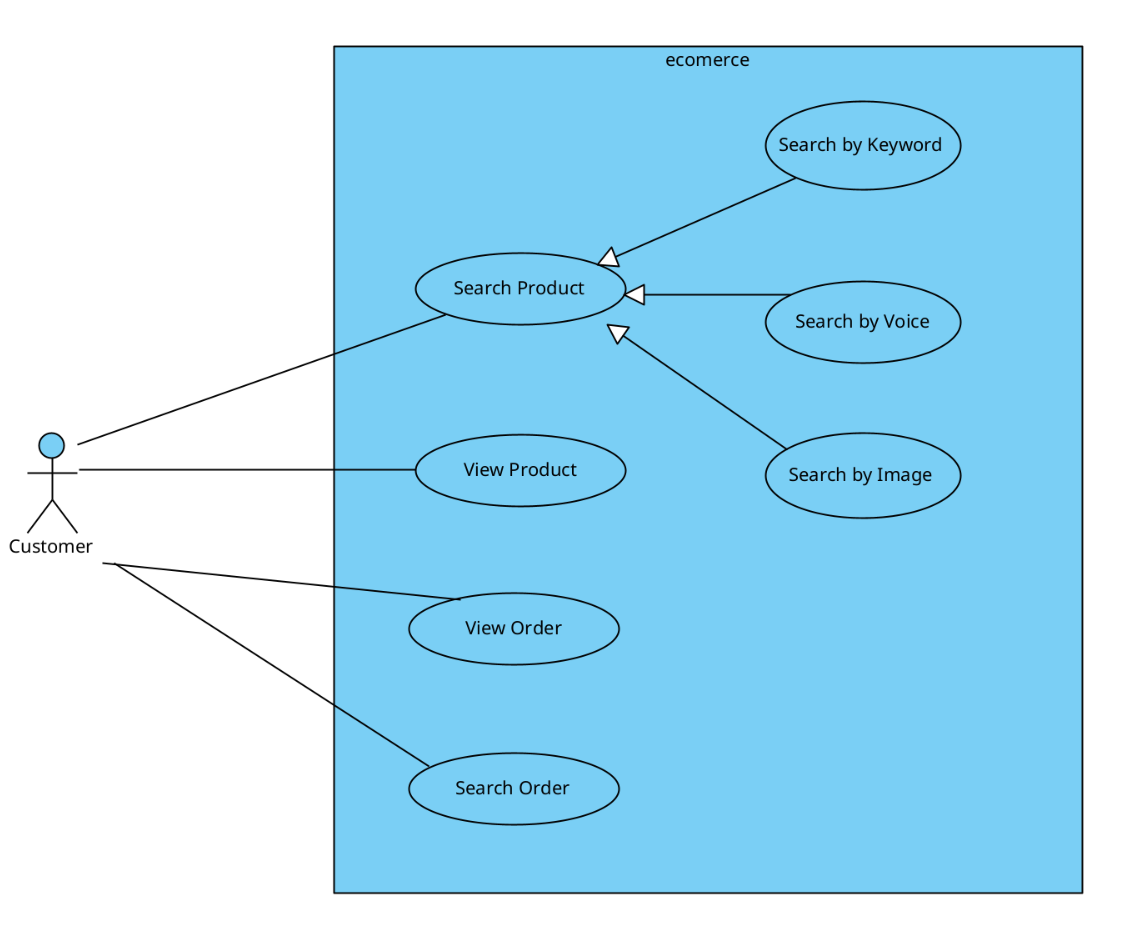
\includegraphics[width=\textwidth,height=0.55\textheight,keepaspectratio]{figures/use-case.png}
\caption{Use case model exported from Visual Paradigm.}\label{fig:usecase}
\end{figure}

The relationship between Search Product and the three modality-specific use cases is modeled using UML generalization (represented by hollow triangular arrows pointing toward Search Product). This signifies that keyword, voice, and image queries share the same fundamental goal of product discovery while specializing the input mechanism. Multimodal search is an integrated composite flow combining text and visual representations.

\subsection{Use case summary and interaction flows}
% Table~\ref{tab:uc} describes the primary product search use cases, highlighting both normal execution and alternative/exception flows.

\begin{table}[H]\centering\small
\caption{Product search use case descriptions.}\label{tab:uc}
\begin{tabularx}{\textwidth}{@{}p{32mm}LL@{}}\toprule
\textbf{Use case} & \textbf{Main flow} & \textbf{Alternative flow} \\\midrule
Search by Keyword & Customer enters text. QueryService normalizes it; SearchService retrieves candidates; RankingService orders results. & Unknown terms produce an empty result state. \\
Search by Voice & Customer records or uploads audio. SpeechService transcribes speech; QueryService builds query; results are returned. & Permission denial, silence, or unreadable audio triggers an error alert. \\
Search by Image & Customer selects/uploads image. ImageService encodes vector; VectorIndex retrieves candidates; RankingService selects top-k. & Corrupted or oversized ($>5$ MB) images are rejected with an error. \\
Search Order & Customer enters order ID or asks for latest order. OrderRepository retrieves records matching customer ID. & Missing orders or orders belonging to other customers return no result. \\
View Product & Customer selects a product card. Details modal displays full specifications, stock, rating, and image download. & Invalid product ID produces an error. \\
View Order & Customer inspects order record. Status, date, items, and total amount are rendered. & Empty view shown if no orders match criteria. \\
\bottomrule\end{tabularx}\end{table}

\FloatBarrier
\section{Three-Layer Architecture}\label{sec:architecture}

\subsection{Architectural overview and component diagram}
The prototype strictly adheres to a three-layer architectural pattern: Presentation Layer, Application / Intelligence Layer, and Data Layer. Figure~\ref{fig:architecture} shows the component architecture modeled in Visual Paradigm.

\begin{figure}[H]\centering
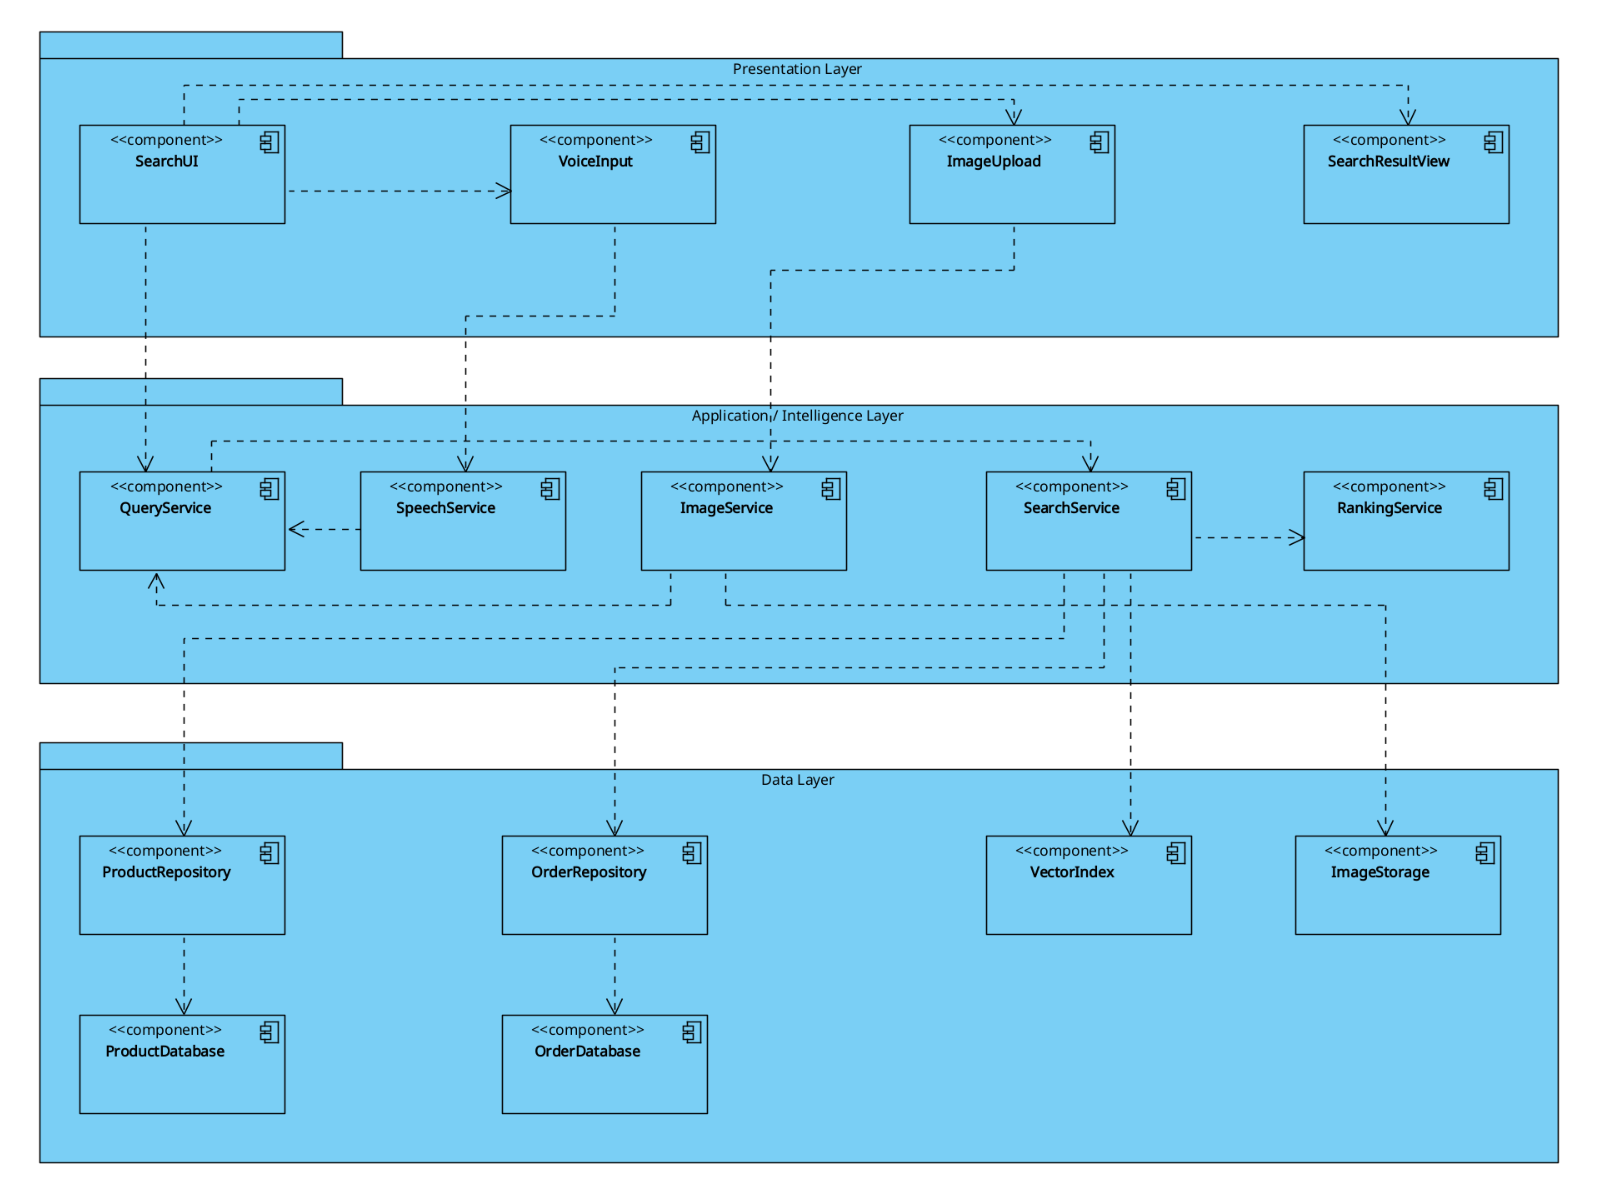
\includegraphics[width=\textwidth,height=0.55\textheight,keepaspectratio]{figures/architecture.png}
\caption{Three-layer component architecture exported from Visual Paradigm.}\label{fig:architecture}
\end{figure}

The dependency direction strictly follows:
\begin{center}
\textbf{Presentation Layer $\longrightarrow$ Application / Intelligence Layer $\longrightarrow$ Data Layer.}
\end{center}
Presentation components never bypass the application layer to access repositories or databases directly ($\text{UI} \not\rightarrow \text{Database}$). This separation ensures business logic remains independent of presentation frameworks and database technologies.

\subsection{Presentation Layer}
The Presentation Layer captures customer inputs and renders formatted responses. In the UML model, it contains SearchUI, VoiceInput, ImageUpload, and SearchResultView. In the Python implementation, this layer comprises:
\begin{itemize}
\item \code{presentation/web\_server.py}: A multithreaded HTTP server implementing RESTful endpoints;
\item \code{presentation/web\_ui.html}: Responsive semantic HTML5 markup based on Bootstrap 5;
\item \code{presentation/static/store.js}: Client-side controller orchestrating microphone recording via the browser MediaRecorder API, drag-and-drop file upload, weight slider events, modal display, and shopping bag persistence;
\item \code{presentation/search\_ui.py}: A command-line interface for terminal-based execution.
\end{itemize}

\subsection{Application / Intelligence Layer}
The Application Layer encapsulates domain logic, query interpretation, AI processing, candidate retrieval, and ranking. Table~\ref{tab:services} details the responsibilities of the five application services.

\begin{table}[htbp]\centering\small
\caption{Application service responsibilities.}\label{tab:services}
\begin{tabularx}{\textwidth}{@{}lL@{}}\toprule
\textbf{Component} & \textbf{Responsibility} \\\midrule
QueryService & Normalizes text, extracts price ceilings, tokenizes words, and constructs common query dictionaries. \\
SpeechService & Transcodes audio using FFmpeg and performs offline speech recognition via Vosk 0.3.45. \\
ImageService & Isolates foreground, crops non-white bounds, and extracts 768-dim RGB feature vectors. \\
SearchService & Manages retrieval pipelines, enforces shared filters (category, price, stock), and fuses scores. \\
RankingService & Sorts candidates by relevance score descending, applies deterministic ID tie-breaking, and selects top-k. \\
\bottomrule\end{tabularx}\end{table}

\subsection{Data Layer and dependency management}
The Data Layer provides persistent storage and data access abstraction:
\begin{itemize}
\item \code{ProductRepository}: Loads \code{data/products.json}, retrieves catalog records, and serves product images;
\item \code{OrderRepository}: Loads \code{data/orders.json} and performs customer-scoped order lookups;
\item \code{VectorIndex}: Maintains precomputed product image descriptors in memory and performs cosine similarity retrieval against query vectors.
\end{itemize}
The composition root in \code{main.py} wires repositories and services at startup, building the image vector index in memory before requests are accepted.

\FloatBarrier
\section{UML Sequence Diagram}\label{sec:sequence}

\subsection{Voice product search sequence}
The sequence diagram models the end-to-end flow of a voice product search. Unlike simulated text pipelines, V02 models genuine audio byte streaming and speech recognition. The participants are Customer, SearchUI, SpeechService, QueryService, SearchService, ProductRepository, and RankingService.

\begin{figure}[H]\centering
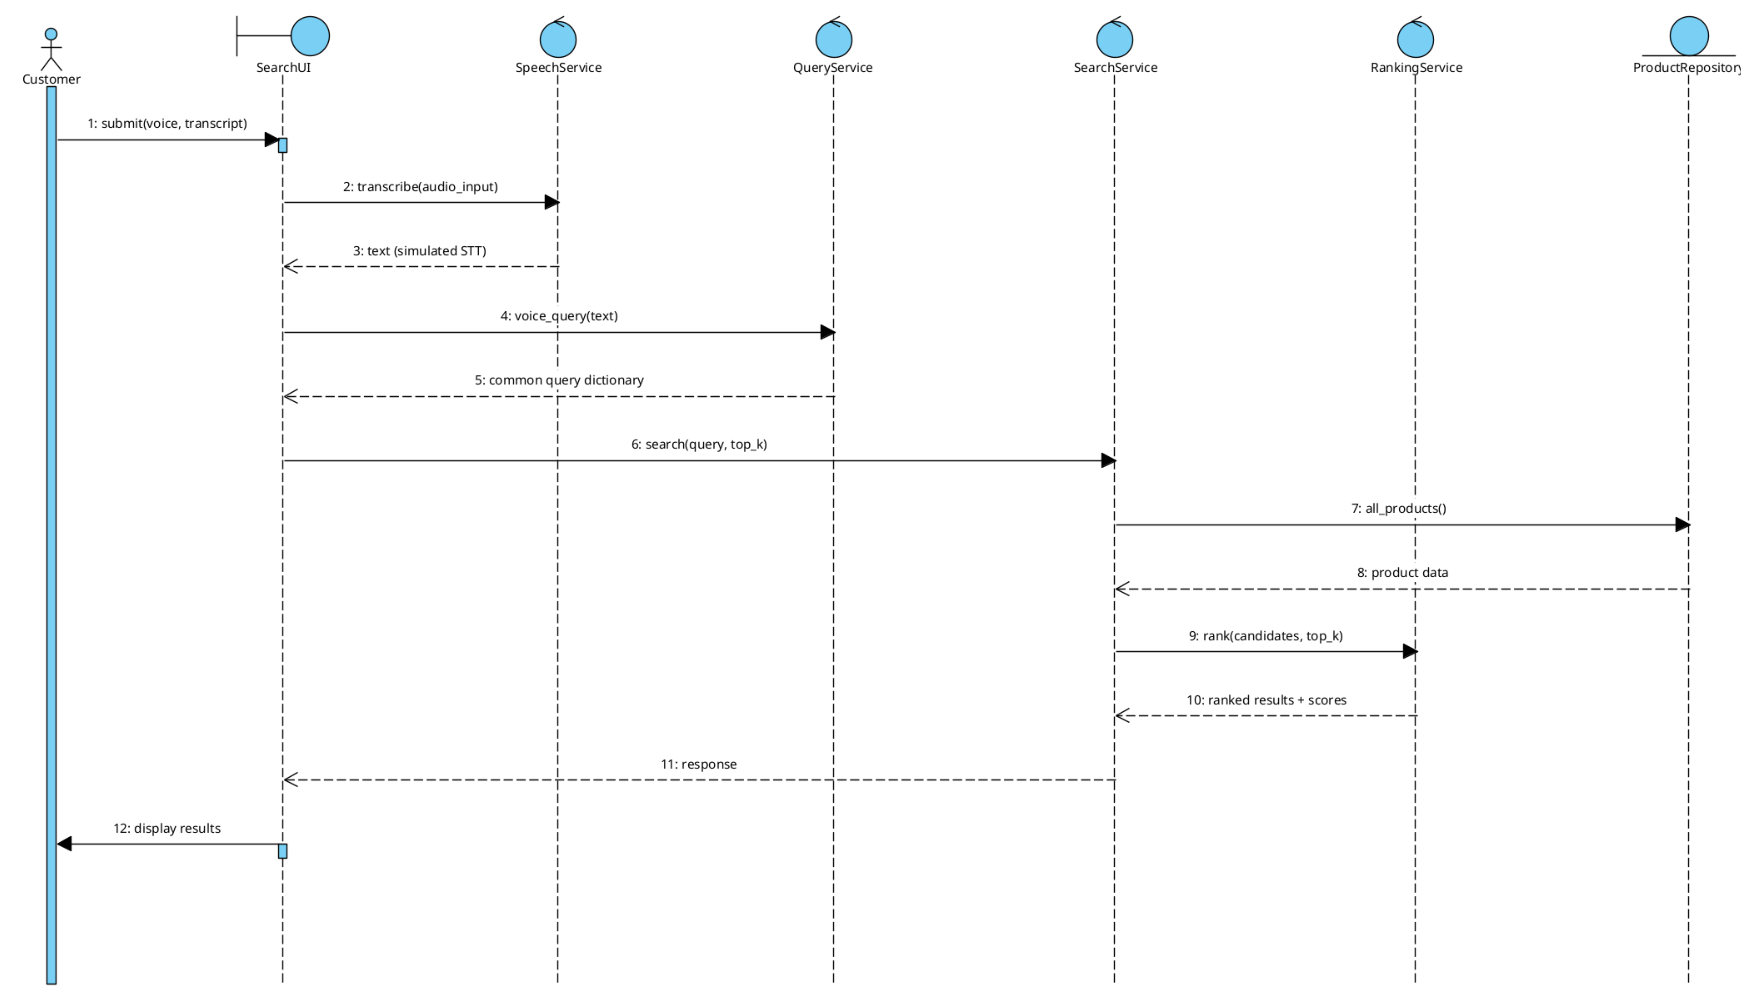
\includegraphics[width=\textwidth,height=0.55\textheight,keepaspectratio]{figures/voice-sequence.png}
\caption{Voice product search sequence diagram exported from Visual Paradigm.}\label{fig:sequence}
\end{figure}

\subsection{Interaction flow}
The execution proceeds through the following numbered interactions:
\begin{enumerate}
\item The Customer clicks \textbf{Start recording} on SearchUI and grants microphone permission.
\item The browser \code{MediaRecorder} captures audio and emits encoded chunks upon clicking \textbf{Stop \& search} (or upon reaching the 12-second limit), releasing microphone hardware tracks immediately.
\item SearchUI transmits the raw audio bytes via \code{POST /api/voice-search} to the HTTP server.
\item SearchUI invokes \code{SpeechService.transcribe\_audio(audio\_bytes)}.
\item SpeechService executes FFmpeg via subprocess to transcode audio into 16 kHz mono 16-bit PCM.
\item SpeechService feeds the PCM stream into the \textbf{offline Vosk} model, returning recognized English text.
\item SearchUI passes the recognized transcript and active customer filters to \code{QueryService.create\_query()}.
\item QueryService normalizes words, extracts price bounds, and builds a common query object with \code{type="voice"}.
\item SearchUI passes the query object to \code{SearchService.search(query)}.
\item SearchService requests candidate product records from \code{ProductRepository.get\_all()}.
\item SearchService applies category, price, and stock predicates, calculating token overlap scores for eligible items.
\item SearchService forwards candidate products and scores to \code{RankingService.rank()}.
\item RankingService sorts candidates by score descending (breaking ties by ascending product ID) and extracts the top-$k$ subset.
\item SearchService returns ranked products and recognized speech metadata to SearchUI.
\item SearchUI renders the recognized transcript, relevance scores, and product cards for the Customer.
\item The Customer views the results or clicks a product card to inspect full specifications.
\end{enumerate}

\FloatBarrier
\section{Python Implementation}\label{sec:implementation}

\subsection{Project organization and execution}
The complete source code and documentation are available in the GitHub repository:\\
\url{https://github.com/KhangDaoz/multimodel-search-system}.

The implementation uses Python 3.10+ (verified on Python 3.14), NumPy for vector operations, Pillow for image manipulation, and Vosk 0.3.45 for speech recognition. FFmpeg is required on PATH for audio conversion.

\begin{lstlisting}[caption={Source code directory layout.}]
multimodel-search-system/
|-- main.py                  # Composition root: wires services & launches server/CLI
|-- evaluate.py              # Automated 30-case evaluation script
|-- presentation/            # Presentation Layer
|   |-- search_ui.py         # Terminal CLI interface
|   |-- web_server.py        # Multithreaded HTTP API server
|   |-- web_ui.html          # Bootstrap 5 storefront markup
|   `-- static/              # CSS, store.js, vendor libraries, assets
|-- application/             # Application / Intelligence Layer
|   |-- query_service.py     # Query normalization & common representation
|   |-- speech_service.py    # Offline Vosk speech-to-text & FFmpeg audio decoding
|   |-- image_service.py     # 768-dim image descriptor extraction & cosine similarity
|   |-- search_service.py    # Candidate retrieval & multimodal score fusion
|   `-- ranking_service.py   # Candidate sorting & deterministic tie-breaking
|-- data/                    # Data Layer
|   |-- products.json        # 15 photographed catalog products
|   |-- orders.json          # Customer order history
|   |-- product_repository.py# Product data access
|   |-- order_repository.py  # Customer-scoped order access
|   |-- vector_index.py      # In-memory vector store & cosine search
|   `-- images/              # Catalog product photos (p01.png - p15.png)
|-- tests/                   # 25 automated unit and HTTP integration tests
|-- tools/                   # Voice model setup and verification scripts
`-- reports/                 # LaTeX report source, figures, and compiled PDF
\end{lstlisting}

The system is executed using the following commands:
\begin{lstlisting}
python -m venv .venv
source .venv/bin/activate
python -m pip install -r requirements.txt
python tools/setup_voice.py       # Downloads official Vosk English model (~40 MB)
python main.py                    # Launches web storefront at http://127.0.0.1:8000
python main.py --cli              # Launches terminal interactive CLI
python main.py --mode audio --query tests/fixtures/blue_shoes.wav
python main.py --mode multimodal --query "blue shoes" \
  --image data/images/p03.png --text-weight 0.7
python -m unittest discover -s tests -v
python evaluate.py
\end{lstlisting}

\subsection{Product repository and service interfaces}
All search modes construct a common query representation dictionary with identical keys:
\begin{lstlisting}[language=Python,caption={Common query dictionary schema.}]
query = {
    "type": "text" | "voice" | "image" | "multimodal",
    "intent": "product" | "order",
    "query": "blue shoes",            # Normalized query string
    "tokens": ["blue", "shoes"],      # Extracted word tokens
    "embedding": [...],               # 768-dim float vector (image/multimodal)
    "filters": {"category": "shoes", "max_price": 100.0, "in_stock": True},
    "customer_id": "C001",            # Scoped demo customer
    "text_weight": 0.7                # Lambda parameter for score fusion
}
\end{lstlisting}

The retrieved candidate products are ordered by \code{RankingService}:
\begin{lstlisting}[language=Python,caption={Ranking and deterministic tie-breaking logic.}]
ranked = sorted(
    candidates,
    key=lambda item: (-item[1], item[0]['id'])
)
return [
    {'product': p, 'score': round(float(s), 6)}
    for p, s in ranked[:top_k]
]
\end{lstlisting}
Candidates are ordered by relevance score descending. When two candidates obtain identical scores, the lower product identifier is ordered first. This deterministic tie-breaking rule ensures repeatable results.

\subsection{Web storefront and request handling}
The FORME storefront interface provides a modern shopping experience:
\begin{itemize}
\item Live microphone capture using the browser MediaRecorder API with real-time waveform visualization;
\item Drag-and-drop or file-selector image upload with preview;
\item Interactive text weight slider ($\lambda \in [0, 1]$) for multimodal fusion;
\item Global filter sidebar (category dropdown, minimum price, maximum price, in-stock checkbox);
\item Product cards displaying genuine photographs, prices, sample ratings, and inventory status;
\item Product details modal with high-resolution image inspection and sample image download;
\item Client-side shopping bag persisting across page reloads via \texttt{localStorage};
\item Customer switcher (C001, C002) for exploring customer-scoped order tracking.
\end{itemize}

\begin{figure}[htbp]\centering
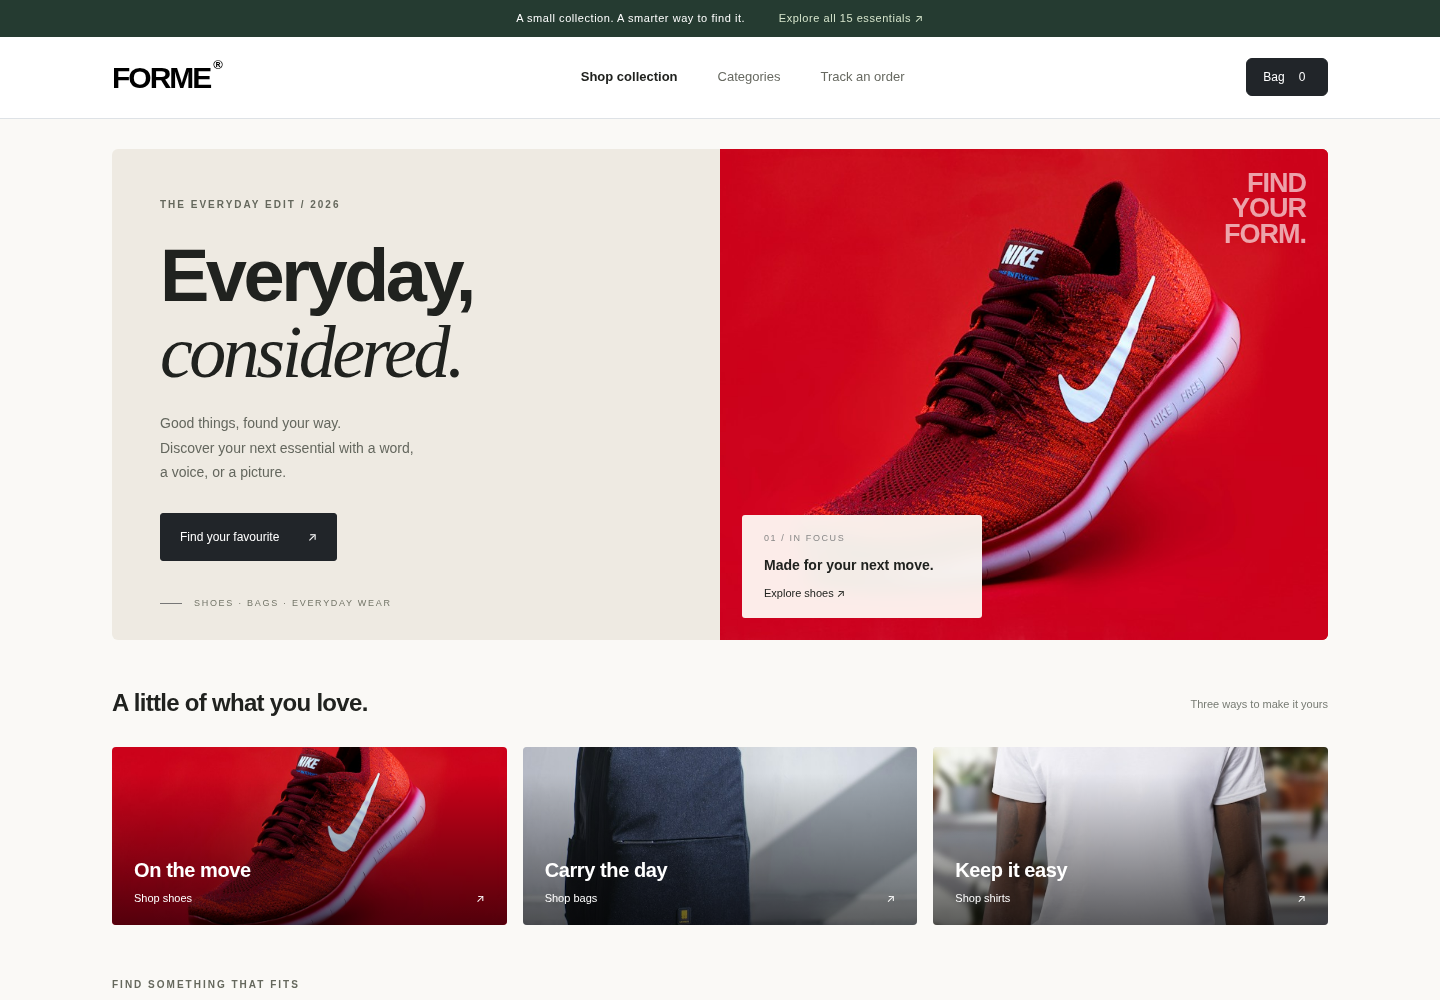
\includegraphics[width=\textwidth,height=0.48\textheight,keepaspectratio]{figures/storefront-overview.png}
\caption{FORME e-commerce web storefront overview showing hero banner, filters, and catalog cards.}\label{fig:overview}
\end{figure}

% Table~\ref{tab:http} enumerates the RESTful API routes provided by \code{presentation/web\_server.py}.

\begin{table}[H]\centering\small
\caption{HTTP routes of the browser application.}\label{tab:http}
\begin{tabularx}{\textwidth}{@{}p{56mm}L@{}}\toprule
\textbf{Route} & \textbf{Purpose} \\\midrule
GET / & Serve the storefront HTML markup and assets. \\
GET /api/catalog & Return filtered catalog products via SearchService. \\
GET /api/products/<id> & Return full specifications of a product from ProductRepository. \\
GET /api/product-images/<id> & Return genuine product photograph bytes. \\
GET /api/voice-status & Report Vosk model readiness and speech recognition availability. \\
POST /api/voice-search & Transcribe raw audio bytes and execute shared search. \\
POST /api/search & Execute text, image, or multimodal query with active filters. \\
GET /static/<path> & Serve local CSS, JavaScript, and vendor libraries. \\
\bottomrule\end{tabularx}\end{table}

% Figure~\ref{fig:demo-cli} illustrates the execution of the command-line prototype across text, audio, image, and multimodal queries.

% \begin{figure}[htbp]\centering
% 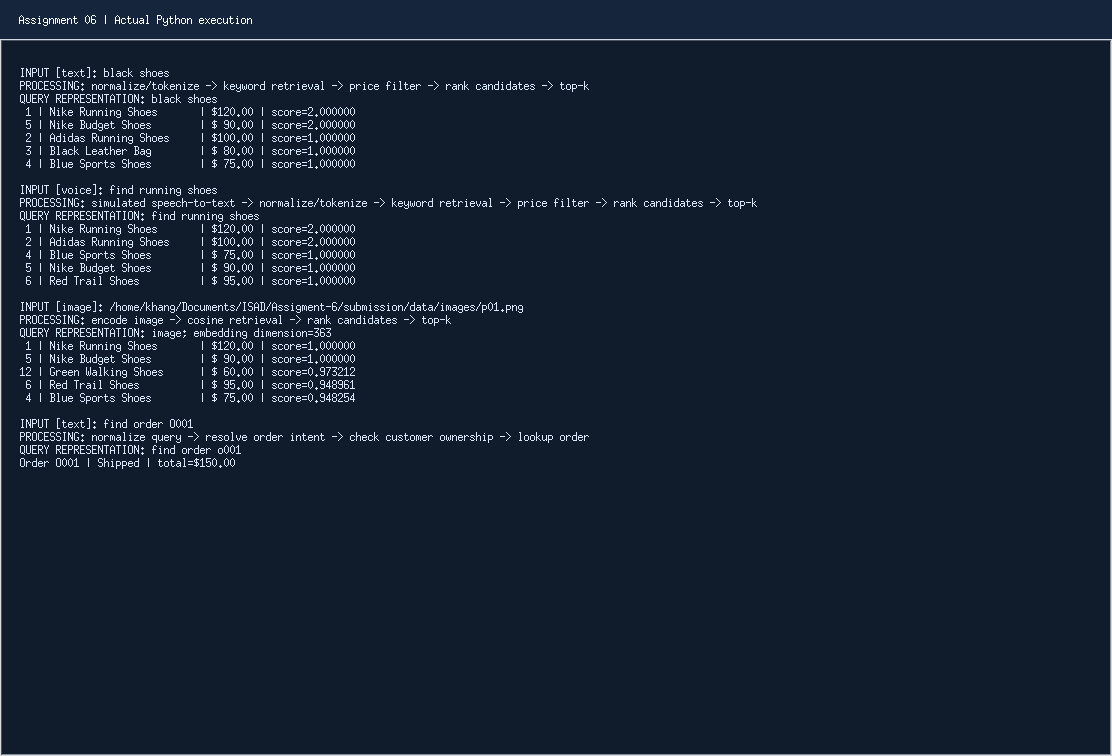
\includegraphics[width=\textwidth,height=0.48\textheight,keepaspectratio]{figures/demo.png}
% \caption{Command-line interface execution demonstration across search modes.}\label{fig:demo-cli}
% \end{figure}

\FloatBarrier
\section{Multimodal Search Method}\label{sec:method}

\subsection{Common query representation}
To support heterogeneous inputs while maintaining architectural simplicity, all search modes converge into the unified query schema defined in Section~\ref{sec:implementation}. The common query object decouples input capture mechanisms from candidate retrieval and ranking.

\subsection{Text and voice search}
Text queries are lowercased and tokenized. Stop words and conversational phrases (``find'', ``show me'', ``please'') are removed. An alias dictionary normalizes common synonyms (e.g., \textit{sneakers}, \textit{trainers} $\rightarrow$ \textit{shoes}; \textit{handbag} $\rightarrow$ \textit{bag}; \textit{dark} $\rightarrow$ \textit{black}).

For query token set $T(q)$ and product word set $W(p)$ (derived from product name, brand, category, color, and description), text relevance is measured as:
\begin{equation}
S_t(p,q) = \frac{|T(q) \cap W(p)|}{\max(|T(q)|, 1)}, \qquad S_t \in [0, 1].
\end{equation}
A candidate must achieve $S_t > 0$ to enter the retrieval set. Normalizing by the query token count ensures text scores reside on a $[0, 1]$ scale directly comparable with visual cosine similarities.

Phrases specifying budget limits (e.g., ``under 100 dollars'') are extracted to enforce a strict price condition:
\begin{equation}
\mathrm{price}(p) < P_{\max}.
\end{equation}
Spoken queries follow this exact pipeline after \code{SpeechService} transcribes speech into text.

\subsection{Image representation and similarity search}
Image similarity search processes photos using a \textbf{handcrafted descriptor}:
\begin{enumerate}
\item EXIF orientation is normalized; transparency channels are composited onto pure white.
\item Images are capped at 20 megapixels to safeguard system resources.
\item A 128-pixel probe detects non-white foreground boundaries, cropping the product subject with padding.
\item The cropped foreground is resized to a $16 \times 16$ RGB canvas.
\item Inverted RGB channel values suppress plain white background influence, generating a $16 \times 16 \times 3 = 768$-dimensional descriptor vector $z$.
\end{enumerate}

\begin{lstlisting}[language=Python,caption={Foreground isolation and 768-dim descriptor extraction.}]
# Crop foreground with padding and fit into 16x16 RGB canvas
cropped = image.crop((left, top, right, bottom))
fitted = fit_foreground(cropped, size=(16, 16))
# Suppress plain white background by inverting normalized RGB values
arr = 1.0 - (np.asarray(fitted, dtype=np.float32) / 255.0)
return arr.reshape(-1) # 768-dimensional float vector
\end{lstlisting}

The cosine similarity between query vector $z_q$ and stored product vector $z_p$ is:
\begin{equation}
S_i(p,q) = \max\left(0, \frac{z_q^\mathsf{T} z_p}{\|z_q\|_2 \|z_p\|_2}\right), \qquad S_i \in [0, 1].
\end{equation}
Zero-norm vectors score zero, and invalid vector dimensions are rejected.

\subsection{Multimodal fusion and final ranking}
When a customer supplies both keywords and a photograph, the representations coexist within the common query dictionary. \code{SearchService} computes a convex combination of both scores:
\begin{equation}
S(p,q) = \lambda S_t(p,q) + (1 - \lambda) S_i(p,q), \qquad \lambda \in [0, 1].
\end{equation}
The parameter $\lambda \in [0, 1]$ represents text importance. At $\lambda = 1$, the ranking reflects pure keyword retrieval; at $\lambda = 0$, it reflects pure image retrieval. Candidates must satisfy all active filters ($p_{\min} \le \text{price} < p_{\max}$, category, in-stock). \code{RankingService} sorts the filtered candidates by score descending, breaking ties by ascending product ID.

\FloatBarrier
\section{Experimental Results}\label{sec:results}

\subsection{Evaluation setup}
The prototype is evaluated using the fixed 30-case test suite in \code{evaluate.py}. Each case specifies an input, search mode, expected top-1 product or order identifier (or empty result), and active filters. The test set comprises 27 functional acceptance cases and 3 explicit limitation probes. Demonstration records are persisted in \code{results/demo.json}, and complete evaluation statistics are stored in \code{results/evaluation.json}.

\subsection{Search demonstrations}
% Table~\ref{tab:demo} presents demonstrations of the primary search modalities.

\begin{table}[htbp]\centering\small
\caption{Saved demonstrations of search modes from results/demo.json.}\label{tab:demo}
\begin{tabularx}{\textwidth}{@{}lLLr@{}}\toprule
\textbf{Mode} & \textbf{Actual input} & \textbf{Top-1 retrieved product} & \textbf{Score} \\\midrule
Text & ``black shoes'' & Nike Air Jordan 1 Red And Black & 1.0000 \\
Voice (audio) & \code{blue\_shoes.wav} (Vosk recognized ``i'm blue shoes'') & Puma Future Rider Trainers & 0.5000 \\
Image & \code{query\_blue\_trainers.png} (rotated/resized query) & Puma Future Rider Trainers & 0.8392 \\
Multimodal & ``blue shoes'' + \code{p03.png}, $\lambda = 0.7$ & Puma Future Rider Trainers & 1.0000 \\
Order & ``find order O001'' (Customer C001) & Order O001 (Total: \$184.98, Status: Shipped) & 1.0000 \\
\bottomrule\end{tabularx}\end{table}

\subsection{Web demonstrations}
The interactive web storefront was verified across all operational modes using automated browser testing. Figures~\ref{fig:web-text}--\ref{fig:web-fusion} present screenshots captured from the running web application on localhost:8000.

% Figure~\ref{fig:web-text} illustrates text search for ``Nike shoes under 100 dollars''. The system parses the budget ceiling, retrieves product 2 (Nike Baseball Cleats at \$79.99), and excludes product 1 (\$149.99).

\begin{figure}[H]\centering
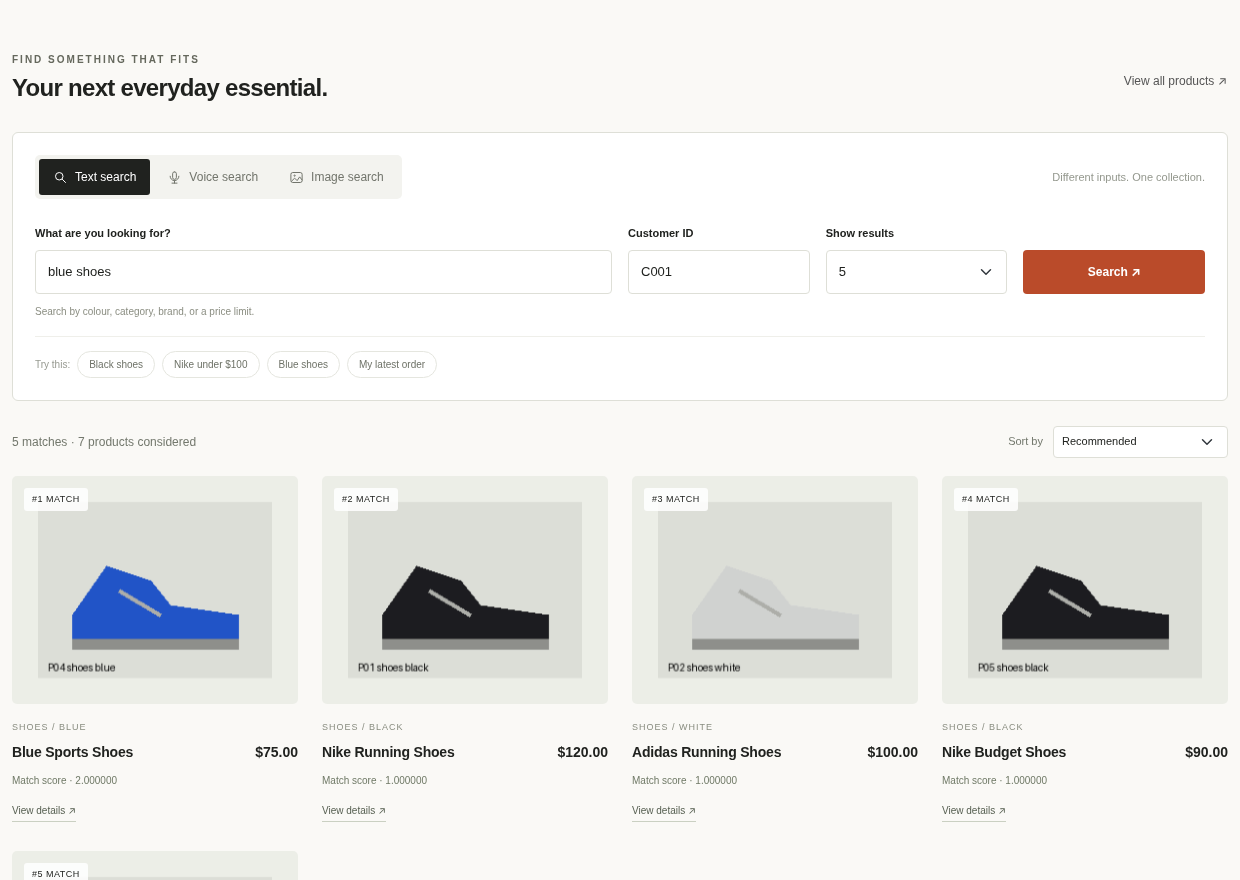
\includegraphics[width=0.92\textwidth,height=0.48\textheight,keepaspectratio]{figures/storefront-search.png}
\caption{Web keyword search for ``Nike shoes under 100 dollars'' with extracted price ceiling filter.}\label{fig:web-text}
\end{figure}

% Figure~\ref{fig:web-voice} displays the live voice search interface, showing the microphone recording modal and audio capture status.H

\begin{figure}[H]\centering
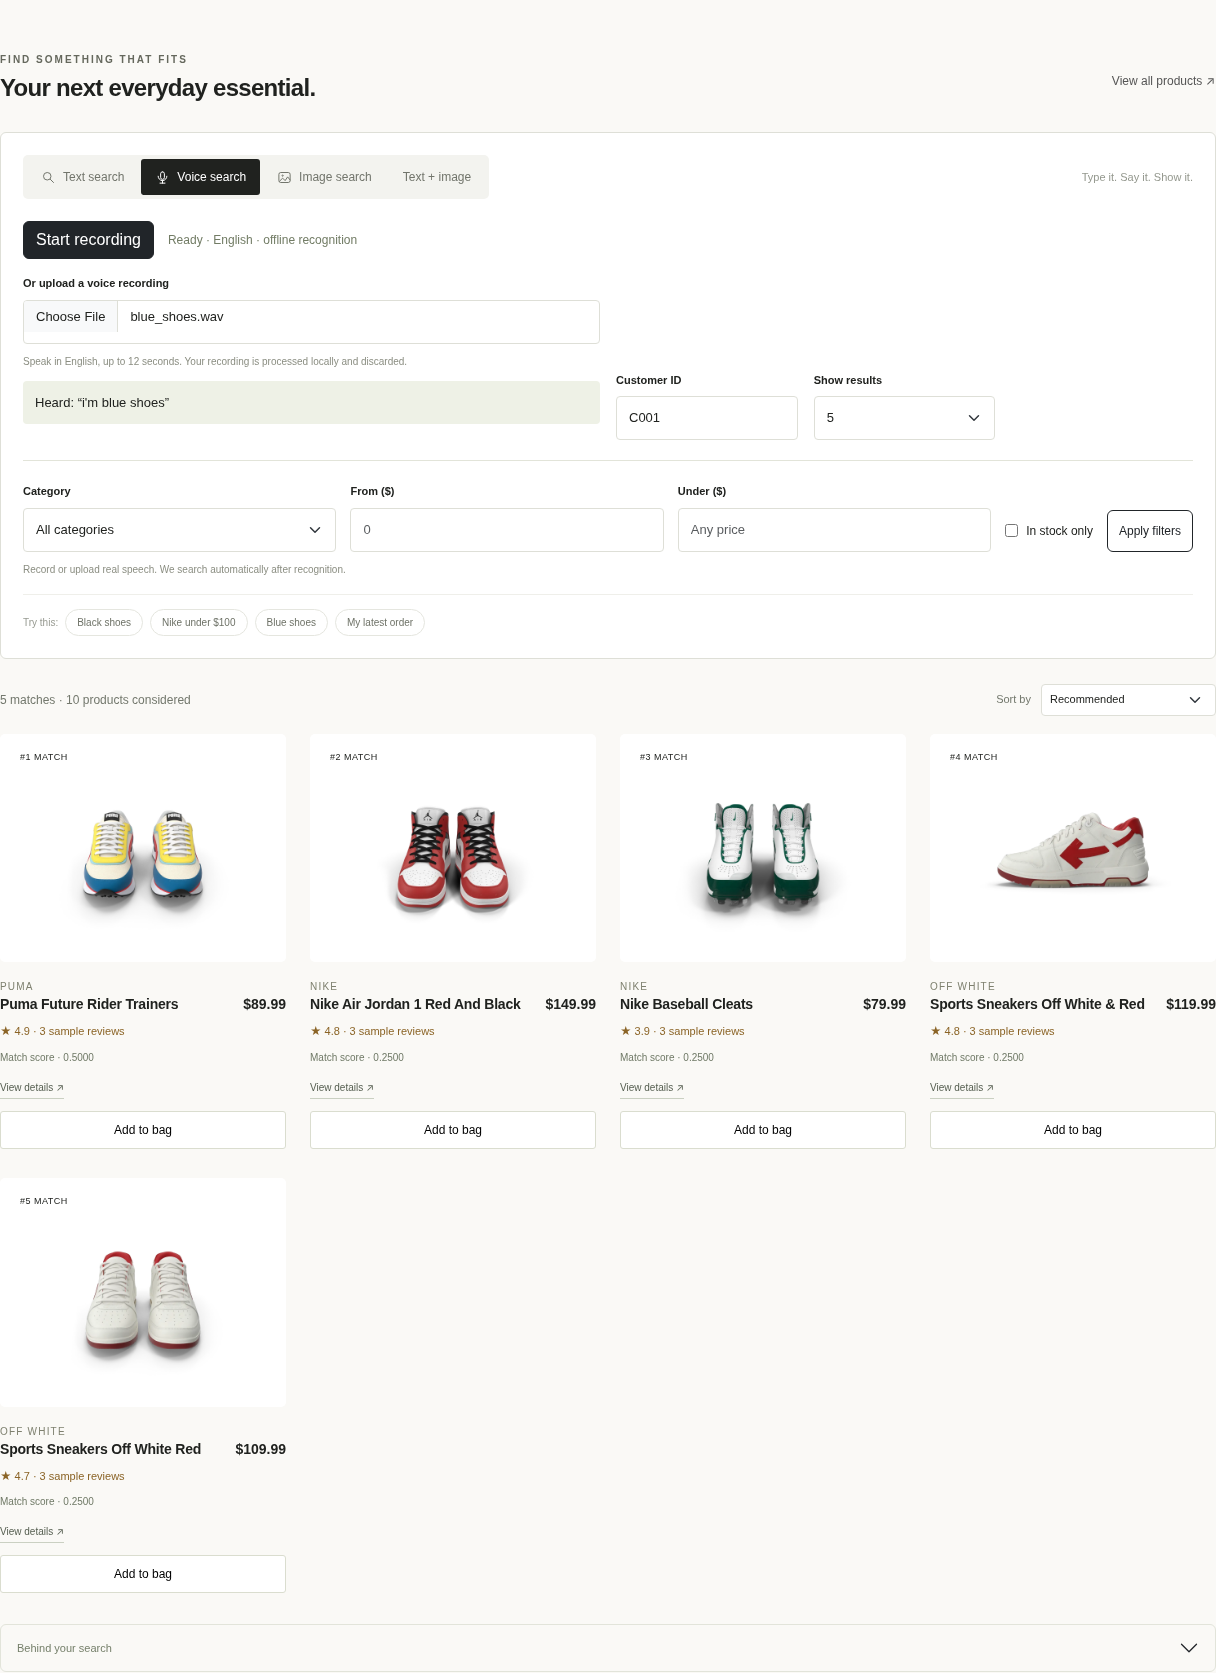
\includegraphics[width=0.92\textwidth,height=0.48\textheight,keepaspectratio]{figures/storefront-voice.png}
\caption{Web voice search recording modal with audio waveform visualization.}\label{fig:web-voice}
\end{figure}

% Figure~\ref{fig:voice-panel} demonstrates the recognized transcript panel after processing speech input, displaying the Vosk recognition result and top matching product.

\begin{figure}[H]\centering
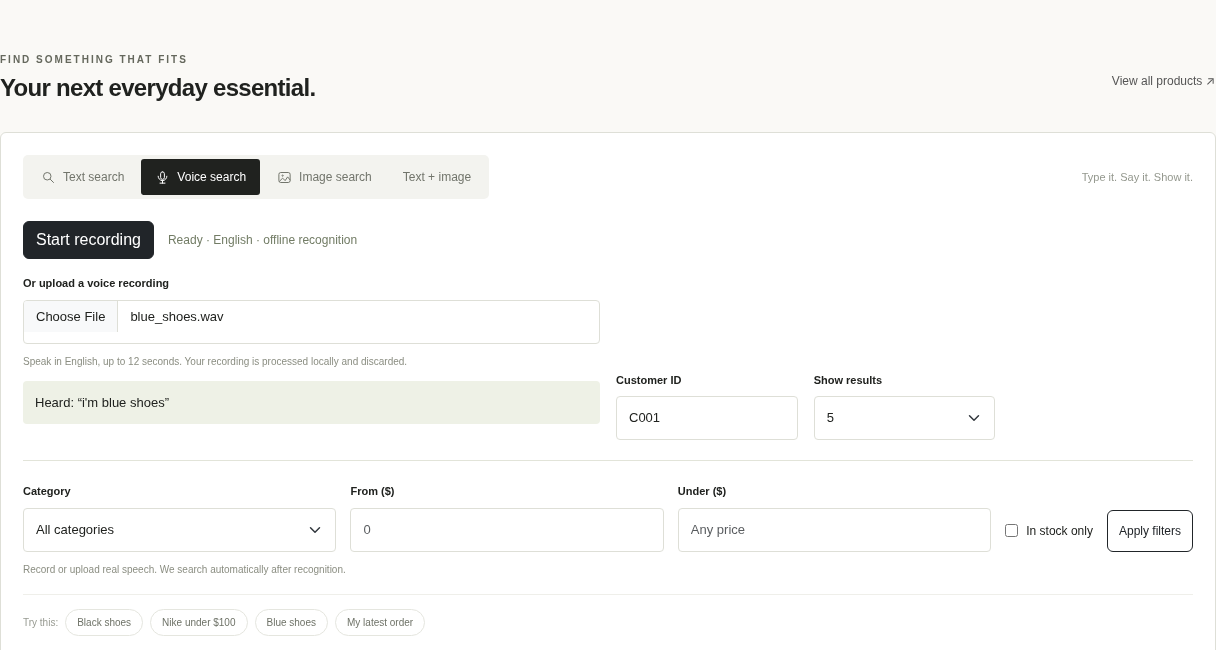
\includegraphics[width=0.92\textwidth,height=0.25\textheight,keepaspectratio]{figures/voice-panel.png}
\caption{Web voice search transcript panel showing recognized text and retrieved product.}\label{fig:voice-panel}
\end{figure}

% Figure~\ref{fig:web-image} illustrates image similarity search. Uploading a product photograph extracts the 768-dim descriptor and ranks catalog items by cosine similarity.

\begin{figure}[H]\centering
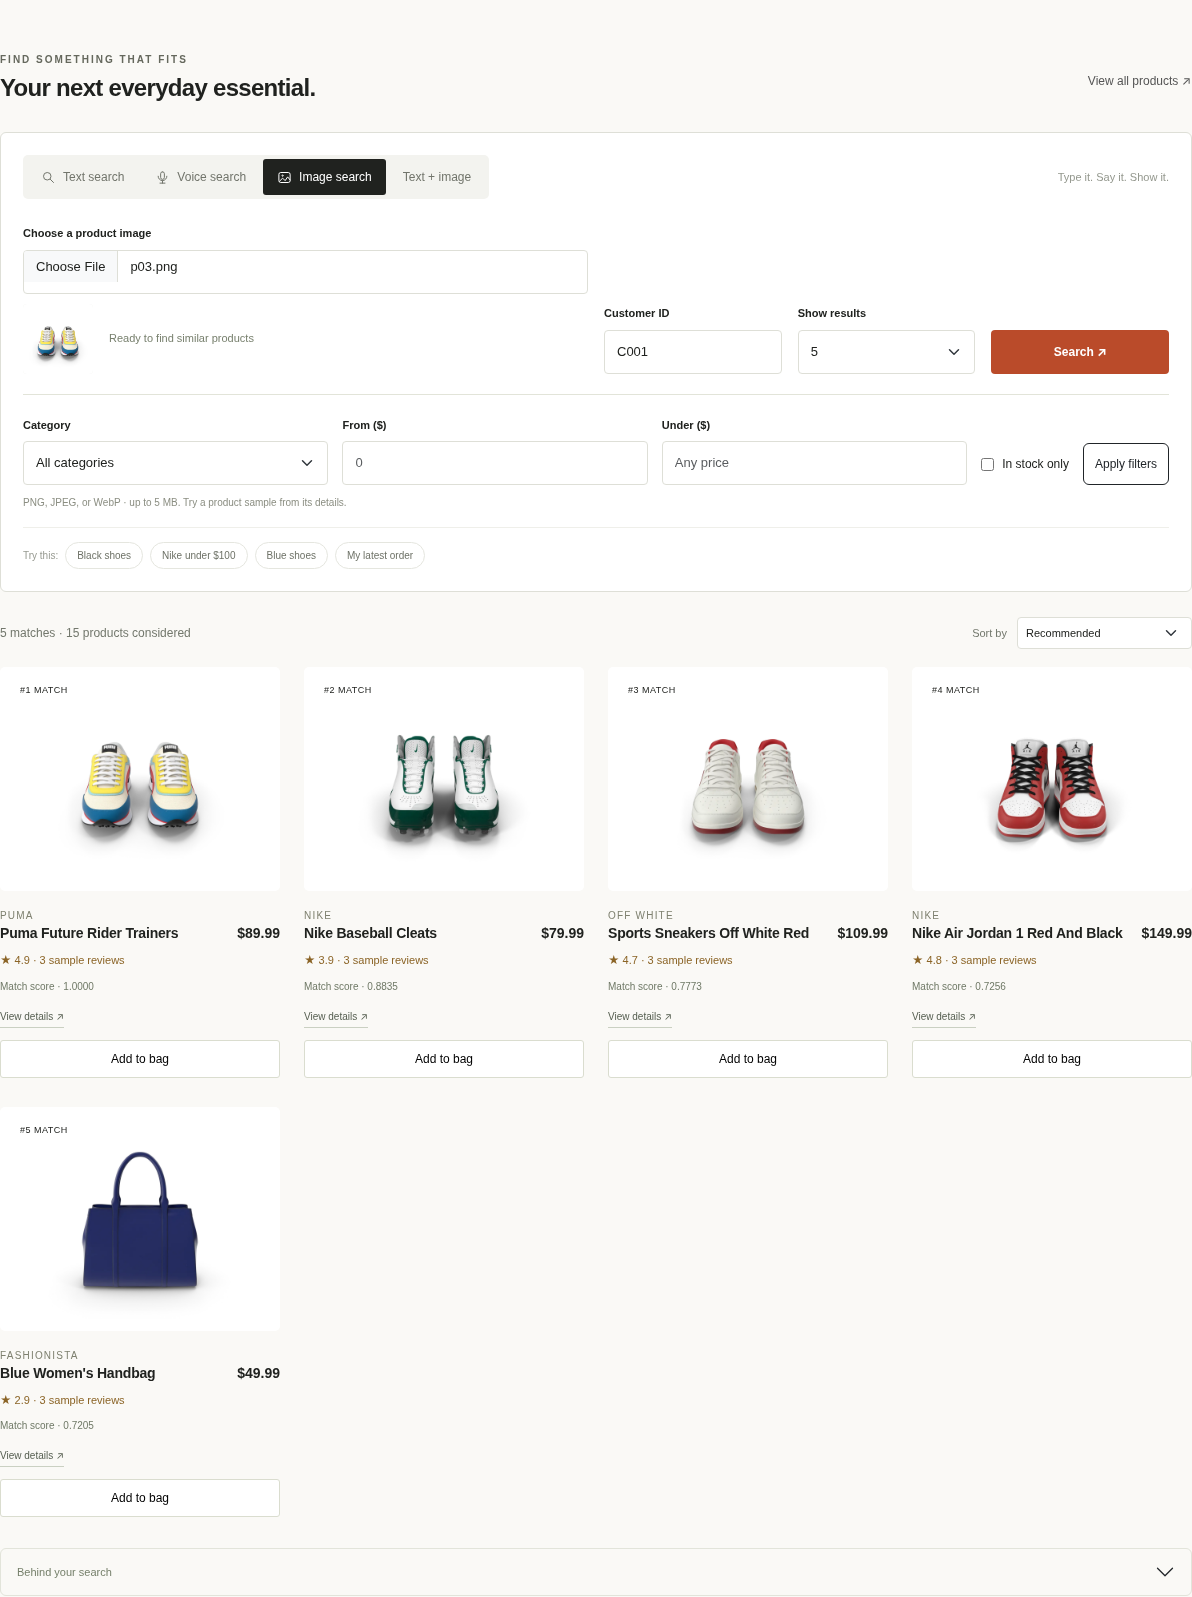
\includegraphics[width=0.92\textwidth,height=0.48\textheight,keepaspectratio]{figures/storefront-image.png}
\caption{Web image search: uploading a product photo retrieves visually matching catalog items.}\label{fig:web-image}
\end{figure}

% Figure~\ref{fig:web-fusion} shows multimodal search combining text keywords with an uploaded image. The customer adjusts the text weight slider ($\lambda$), and product cards display the individual text and image score contributions.

\begin{figure}[H]\centering
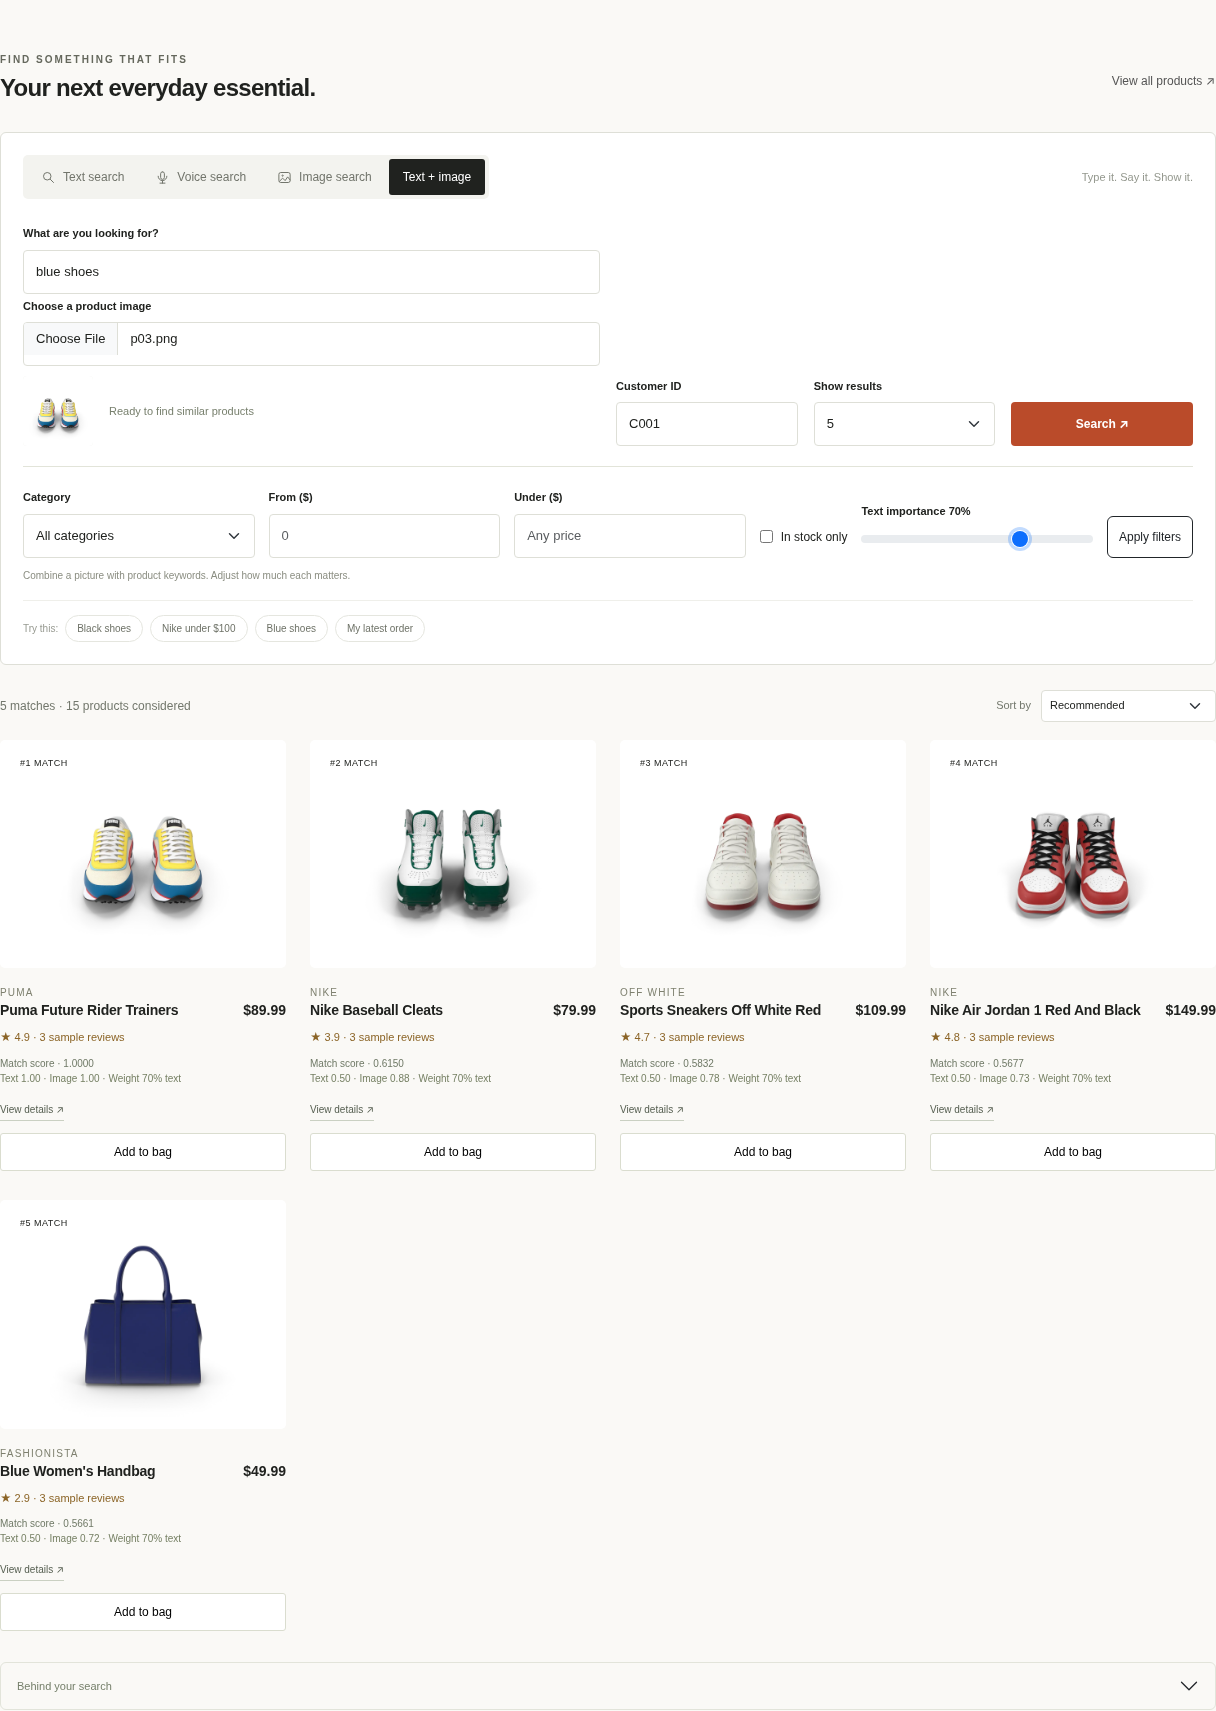
\includegraphics[width=0.92\textwidth,height=0.48\textheight,keepaspectratio]{figures/storefront-fusion.png}
\caption{Web multimodal search combining image upload with text keywords and interactive weight slider.}\label{fig:web-fusion}
\end{figure}

% Figure~\ref{fig:desktop-full} provides a comprehensive view of the responsive desktop storefront.

\begin{figure}[H]\centering
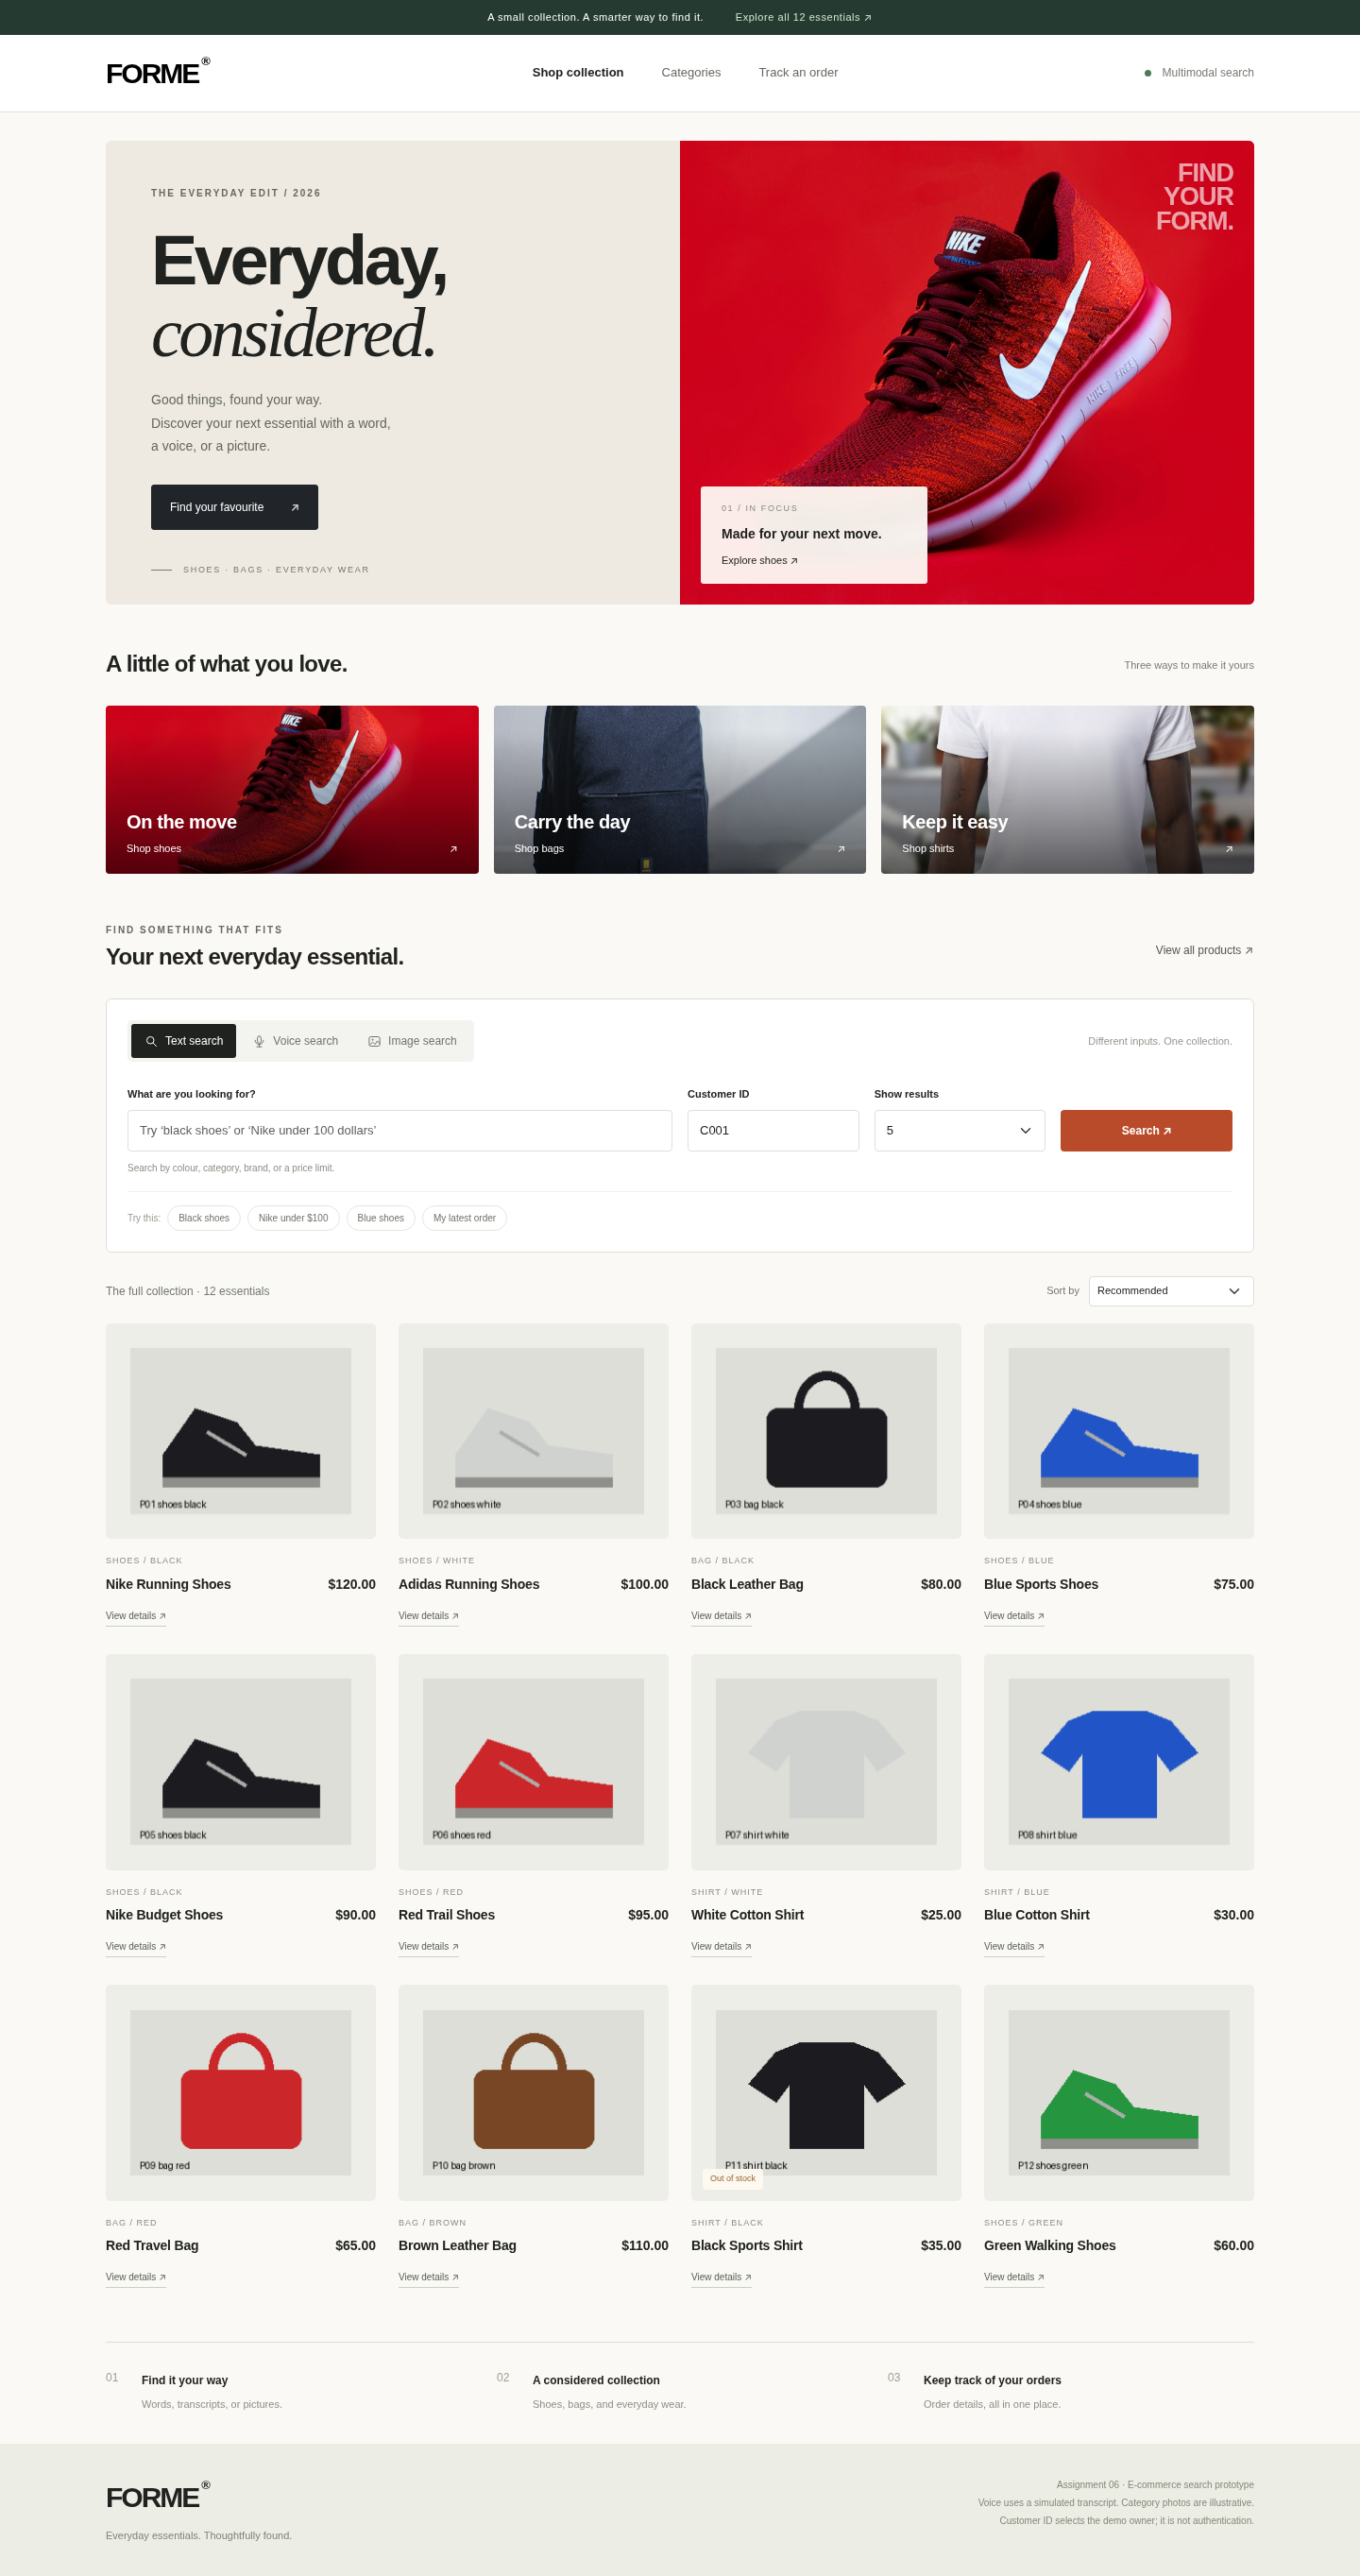
\includegraphics[width=0.92\textwidth,height=0.55\textheight,keepaspectratio]{figures/storefront-desktop.png}
\caption{Full desktop storefront view captured from the running application.}\label{fig:desktop-full}
\end{figure}

\subsection{Evaluation outcomes and failure analysis}
Out of 30 test cases, 28 succeed, yielding an overall success rate of \textbf{93.33\%} (and 100\% on functional acceptance cases).
\begin{equation}
\mathrm{Success\ Rate} = \frac{28}{30} \times 100\% = 93.33\%.
\end{equation}

% Table~\ref{tab:mode-results} groups outcomes and average response times by search modality.

\begin{table}[H]\centering\small
\caption{Experimental test outcomes grouped by input modality.}\label{tab:mode-results}
\begin{tabular}{@{}lrrrr@{}}\toprule
\textbf{Mode} & \textbf{Total queries} & \textbf{Successful} & \textbf{Success rate} & \textbf{Avg latency (ms)} \\\midrule
Text & 20 & 19 & 95.00\% & 0.17 ms \\
Image & 5 & 5 & 100.00\% & 19.98 ms \\
Multimodal & 3 & 3 & 100.00\% & 26.20 ms \\
Audio & 2 & 1 & 50.00\% & 889.75 ms \\\midrule
\textbf{Total / Overall} & \textbf{30} & \textbf{28} & \textbf{93.33\%} & \textbf{61.91 ms} \\
\bottomrule\end{tabular}\end{table}

% Table~\ref{tab:failures} analyzes the two failed test cases, which were intentionally included to characterize system limitations.

\begin{table}[H]\centering\small
\caption{Retained failed cases and failure analysis.}\label{tab:failures}
\begin{tabularx}{\textwidth}{@{}LLrr@{}}\toprule
\textbf{Input} & \textbf{Failure analysis / Explanation} & \textbf{Expected} & \textbf{Actual} \\\midrule
\code{black\_bag.wav} & Speech recognition robustness probe: synthetic voice audio was misrecognized as ``black man'' instead of ``black bag'', causing product 1 to match rather than bag 15. & 15 & 1 \\
``black shoes'' & Unstated budget preference probe: expects cheaper shoe, but query specifies no price preference; V02 intentionally uses explicit filters rather than arbitrary price bias. & 2 & 1 \\
\bottomrule\end{tabularx}\end{table}

Additionally, all 25 automated unit and integration tests pass successfully in \code{results/tests.txt}, and 19/19 browser verification checks pass without JavaScript exceptions.

\FloatBarrier
\section{Discussion}\label{sec:discussion}

\subsection{Design assessment and observed strengths}
The V02 prototype demonstrates high architectural integrity. The three-layer design cleanly decouples user interface concerns from business logic and data persistence. Key strengths include:
\begin{itemize}
\item Genuine offline speech recognition via Vosk and FFmpeg eliminates dependencies on mock transcripts;
\item Authenticated catalog data with high-resolution photography replaces synthetic placeholder images;
\item Multimodal score fusion with an interactive weight slider offers transparent and explainable result ranking;
\item Global multi-attribute filters apply uniformly across text, voice, image, and multimodal retrieval;
\item Candidate retrieval is strictly separated from ranking (Principle 3), with deterministic ID tie-breaking;
\item Client-side shopping bag state in \texttt{localStorage} provides a complete user experience.
\end{itemize}

\subsection{Limitations}
\begin{itemize}
\item \textbf{Handcrafted Visual Descriptor:} The 768-dim color-spatial descriptor is sensitive to lighting, camera angles, and background variations. It lacks the deep semantic invariance of modern vision models (e.g., CLIP).
\item \textbf{Acoustic Robustness:} The lightweight Vosk English model may misrecognize heavily accented, noisy, or synthetically synthesized speech (as observed in the \code{black\_bag.wav} probe).
\item \textbf{Rule-Based Synonym Matching:} Keyword matching relies on token overlap and a finite alias dictionary rather than learned semantic language embeddings.
\item \textbf{Data Scope:} Catalogs and orders are managed via local JSON files without multi-tenant authentication or database transactions.
\end{itemize}

% \subsection{Possible improvements}
% Future development can enhance the system by:
% \begin{itemize}
% \item Replacing handcrafted descriptors with pretrained multimodal embeddings (e.g., CLIP, SigLIP) to project text and images into a shared semantic vector space;
% \item Adopting a dedicated vector database (e.g., Milvus, Qdrant, or PostgreSQL with pgvector);
% \item Supporting multilingual speech models and noise-filtering preprocessors;
% \item Implementing full user authentication and persistent order management.
% \end{itemize}

% \begin{table}[htbp]\centering\small
% \caption{Evidence-based self-assessment against assignment Table 4 rubric.}\label{tab:rubric}
% \begin{tabularx}{\textwidth}{@{}Lrr@{}}\toprule
% \textbf{Rubric component} & \textbf{Max points} & \textbf{Self-assessed} \\\midrule
% Requirements analysis & 10 & 10 \\
% Use Case Diagram & 15 & 14 \\
% Three-Layer Architecture & 20 & 19 \\
% Sequence Diagram & 10 & 9 \\
% Python implementation & 20 & 19 \\
% Multimodal search & 10 & 9 \\
% Experimental evaluation & 5 & 5 \\
% Report quality & 5 & 4 \\
% Demonstration & 5 & 5 \\\midrule
% \textbf{Total Score} & \textbf{100} & \textbf{94} \\
% \bottomrule\end{tabularx}\end{table}

\FloatBarrier
\section{Conclusion}\label{sec:conclusion}
This assignment designed, modeled, implemented, and evaluated a multimodal search system for e-commerce. The project demonstrates how heterogeneous inputs—text keywords, spoken audio, and product images—can be transformed into a unified query representation, filtered according to shared business constraints, and ranked effectively within a three-layer software architecture.

The deliverables include Visual Paradigm UML models, a Python prototype with real offline speech recognition and multimodal fusion, an authentic 15-product catalog, automated test suites, and empirical evaluation records. The architecture provides a solid, maintainable foundation for incorporating production-grade AI models in future iterations.

\subsection*{References}
\begin{enumerate}[label={[\arabic*]}]
\item D. Q. Tran, \textit{Assignment 06: Multimodal Search System for E-Commerce}, Faculty of Information Technology I, Posts and Telecommunications Institute of Technology, 2026.
\item Alpha Cephei, \textit{Vosk Offline Speech Recognition API}, \url{https://alphacephei.com/vosk/}.
\item W3C, \textit{MediaStream Recording API}, \url{https://w3c.github.io/mediacapture-record/}.
\item DummyJSON, \textit{E-Commerce Products Dataset}, \url{https://dummyjson.com/products}.
\item Bootstrap Team, \textit{Bootstrap 5 Documentation}, \url{https://getbootstrap.com/}.
\item Đào Văn Khang, \textit{Multimodal Search System Repository}, \url{https://github.com/KhangDaoz/multimodel-search-system}.
\end{enumerate}

\end{document}
